\section{ Tok manbalarini ketma-ket va parallel ulash.}



\begin{enumerate}

\item EYK’i $6$ V, ichki qarshiligi $2~\Omega$ bo‘lgan $10$ ta doimiy tok manbai ketma-ket ulangan. Zanjirning to‘la EYKini toping (V).
\begin{enumerate}[label=\Alph*)]
\item 0,6.
\item 6.
\item 12.
\item 120.
\item 60.
\end{enumerate}

\item Har birining EYK $2$ V, ichki qarshiligi $0,3~\Omega$ bo‘lgan $6$ ta element qarshiligi $1,2~\Omega$ bo‘lgan tashqi zanjirga ketma-ket ulangan. Zanjirdagi tok kuchi qanday (A)?
\begin{enumerate}[label=\Alph*)]
\item 3,2.
\item $4/3$.
\item 3,6.
\item 2.
\item 4.
\end{enumerate}

\item EYK’i $3$ V va ichki qarshiligi $2~\Omega$ dan bo‘lgan $6$ ta bir xil element ketma-ket ulanib, batareya hosil qilingan. Agar shu batareyaga $6~\Omega$ tashqi qarshilik ulangan bo‘lsa, unda qanday tok kuchi hosil bo‘ladi (A)?
\begin{enumerate}[label=\Alph*)]
\item 3.
\item 2.
\item 1,5.
\item 1.
\item 0,5.
\end{enumerate}

\item EYK’i $6$ V va ichki qarshiligi $1~\Omega$ dan bo‘lgan $10$ ta tok manbai o‘zaro ketma-ket ulanib, batareya hosil qilingan. Agar bu batareyaga qarshiligi $5~\Omega$ bo‘lgan rezistor ulansa, undagi tok kuchi qanday (A)?
\begin{enumerate}[label=\Alph*)]
\item 6.
\item 4.
\item 3.
\item 2.
\item 1.
\end{enumerate}

\item Har birining EYK’i $6$ V va ichki qarshiligi $0,6~\Omega$ bo‘lgan ikkita akkumulator ketma-ket ulanganda, $2$ A tok bo‘lishi uchun tashqi zanjirdagi qarshilik qanday bo‘lishi kerak ($\Omega$)?
\begin{enumerate}[label=\Alph*)]
\item 48.
\item 18.
\item 4,8.
\item 2.
\item 0,48.
\end{enumerate}

\item Tashqi zanjirdagi kuchlanish $100$ V va tok kuchi $5$ A bo‘lishi uchun EYK’i $2,5$ V va ichki qarshiligi $0,1~\Omega$ dan bo‘lgan manbalardan nechtasini ketma-ket ulab, batareya tuzish kerak?
\begin{enumerate}[label=\Alph*)]
\item 25.
\item 36.
\item 38.
\item 40.
\item 50.
\end{enumerate}

\item Rasmda ko‘rsatilgan elektr zanjirda $\varepsilon_1=6$ V, $\varepsilon_2=18$ V, $R=3~\Omega$. Manbalar ichki qarshilikka ega emas. Zanjirdagi tok kuchi necha Amper?

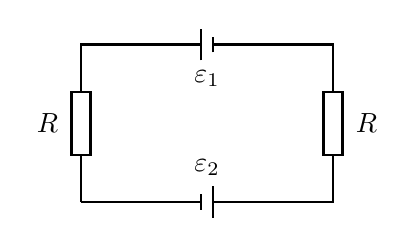
\begin{tikzpicture}[thick, xscale=0.8]
    % To'rtburchak zanjir asosi
    \draw (0,0) -- (0,2) -- (4,2) -- (4,0) -- (0,0);

    % Yuqorigi tok manbai (E1)
    \fill[white] (1.9,1.9) rectangle (2.1,2.1);
    \draw (1.9,1.8) -- (1.9,2.2); % Uzun chiziq (+)
    \draw (2.1,1.9) -- (2.1,2.1); % Qisqa chiziq (-)
    \node[below] at (2,1.8) {$\varepsilon_1$};

    % Pastki tok manbai (E2)
    \fill[white] (1.9,-0.1) rectangle (2.1,0.1);
    \draw (1.9,-0.1) -- (1.9,0.1); % Qisqa chiziq (-)
    \draw (2.1,-0.2) -- (2.1,0.2); % Uzun chiziq (+)
    \node[above] at (2,0.2) {$\varepsilon_2$};

    % Chap tomondagi rezistor (R)
    \fill[white] (-0.2,0.6) rectangle (0.2,1.4);
    \draw (-0.15,0.6) rectangle (0.15,1.4);
    \node[left] at (-0.2,1) {$R$};

    % O'ng tomondagi rezistor (R)
    \fill[white] (3.8,0.6) rectangle (4.2,1.4);
    \draw (3.85,0.6) rectangle (4.15,1.4);
    \node[right] at (4.2,1) {$R$};

\end{tikzpicture}

\begin{enumerate}[label=\Alph*)]
\item 8.
\item 6.
\item 4.
\item 3.
\item 2.
\end{enumerate}

\item $\varepsilon_1=5$ V, $\varepsilon_2=3$ V, $\varepsilon_3=4$ V, $r=1~\Omega$ va $R=7~\Omega$ bo‘lsa, $R$ qarshilikdagi kuchlanish tushishi necha Volt bo‘ladi (rasmga q.)?

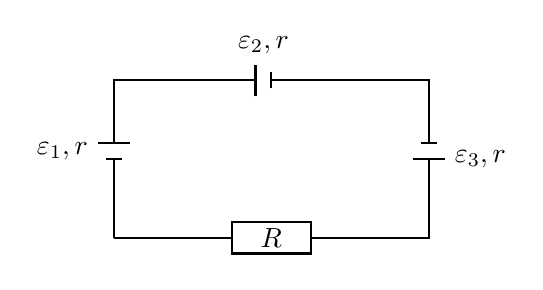
\begin{tikzpicture}[thick, scale=1]
    % To'rtburchak zanjir asosi
    \draw (0,0) -- (0,2) -- (4,2) -- (4,0) -- (0,0);

    % Chap tomondagi tok manbai (E1)
    \fill[white] (-0.1,1) rectangle (0.1,1.2);
    \draw (-0.2,1.2) -- (0.2,1.2); % Uzun chiziq (+)
    \draw (-0.1,1) -- (0.1,1); % Qisqa chiziq (-)
    
    \node[left] at (-0.2,1.1) {$\varepsilon_1, r$};

    % Yuqorigi tok manbai (E2)
    \fill[white] (1.8,1.9) rectangle (2,2.1);
    \draw (1.8,1.8) -- (1.8,2.2); % Uzun chiziq (+)
    \draw (2,1.9) -- (2,2.1); % Qisqa chiziq (-)
    \node[above] at (1.9,2.2) {$\varepsilon_2, r$};

    % O'ng tomondagi tok manbai (E3)
    \fill[white] (3.9,1) rectangle (4.1,1.2);
    \draw (3.8,1) -- (4.2,1); % Uzun chiziq (+)
    \draw (3.9,1.2) -- (4.1,1.2); % Qisqa chiziq (-)
    \node[right] at (4.2,1) {$\varepsilon_3, r$};

    % Pastki tomondagi rezistor (R)
    \fill[white] (1.5,-0.3) rectangle (2.5,0.3);
    \draw (1.5,-0.2) rectangle (2.5,0.2) node[midway] {$R$};

\end{tikzpicture}

\begin{enumerate}[label=\Alph*)]
\item 14.
\item 1,4.
\item 7.
\item 0,7.
\item 8,4.
\end{enumerate}

\item Sxemada $\varepsilon_1=9$ V, $\varepsilon_2=6$ V va $R_1/R_2=2$ bo‘lsa, $R_2$ qarshilikdagi kuchlanish tushishi necha Volt bo‘ladi? Manbalarning ichki qarshiliklari $r_1=r_2=0$.

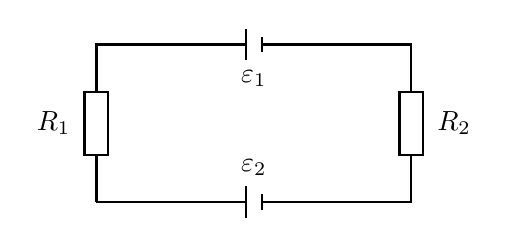
\begin{tikzpicture}[thick, scale=1]
    % To'rtburchak zanjir asosi
    \draw (0,0) -- (0,2) -- (4,2) -- (4,0) -- (0,0);

    % Yuqorigi tok manbai (E1)
    \fill[white] (1.9,1.9) rectangle (2.1,2.1);
    \draw (1.9,1.8) -- (1.9,2.2); % Uzun chiziq (+)
    \draw (2.1,1.9) -- (2.1,2.1); % Qisqa chiziq (-)
    \node[below] at (2,1.8) {$\varepsilon_1$};

    % Pastki tok manbai (E2)
    \fill[white] (1.9,-0.1) rectangle (2.1,0.1);
    \draw (1.9,-0.2) -- (1.9,0.2); % Uzun chiziq (+)
    \draw (2.1,-0.1) -- (2.1,0.1); % Qisqa chiziq (-)
    \node[above] at (2,0.2) {$\varepsilon_2$};

    % Chap tomondagi rezistor (R1)
    \fill[white] (-0.2,0.6) rectangle (0.2,1.4);
    \draw (-0.15,0.6) rectangle (0.15,1.4);
    \node[left] at (-0.2,1) {$R_1$};

    % O'ng tomondagi rezistor (R2)
    \fill[white] (3.8,0.6) rectangle (4.2,1.4);
    \draw (3.85,0.6) rectangle (4.15,1.4);
    \node[right] at (4.2,1) {$R_2$};

\end{tikzpicture}

\begin{enumerate}[label=\Alph*)]
\item 3.
\item 2.
\item 1.
\item 5.
\item 7,5.
\end{enumerate}

\item Rasmda ko‘rsatilgan elektr zanjirda $\varepsilon_1=6$ V, $\varepsilon_2=12$ V va $R=6~\Omega$. Manbalarning ichki qarshiligi bo‘lmasa, zanjirdagi tok kuchi necha Amper bo‘ladi?

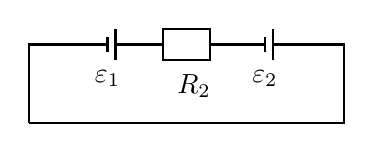
\begin{tikzpicture}[thick, scale=1]
    % To'rtburchak zanjir asosi
    \draw (0,1) -- (0,2) -- (4,2) -- (4,1) -- (0,1);

    % Yuqorigi tok manbai (E1) - Qutblari: - | +
    \fill[white] (1,1.9) rectangle (1.1,2.1);
    \draw (1,1.9) -- (1,2.1); % Qisqa chiziq (-)
    \draw (1.1,1.8) -- (1.1,2.2); % Uzun chiziq (+)
    \node[below] at (1,1.8) {$\varepsilon_1$};

     % Yuqorigi tok manbai (E1) - Qutblari: - | +
    \fill[white] (3,1.9) rectangle (3.1,2.1);
    \draw (3,1.9) -- (3,2.1); % Qisqa chiziq (-)
    \draw (3.1,1.8) -- (3.1,2.2); % Uzun chiziq (+)
    \node[below] at (3,1.8) {$\varepsilon_2$};
    

        % O'ng tomondagi rezistor (R2)
    \fill[white] (1.7,1.9) rectangle (2.3,2.1);
    \draw (1.7,1.8) rectangle (2.3,2.2);
    \node[above] at (2.1,1.2) {$R_2$};

\end{tikzpicture}

\begin{enumerate}[label=\Alph*)]
\item 1.
\item 2.
\item 3.
\item 4.
\item 0.
\end{enumerate}

\item Rasmda ko‘rsatilgan elektr zanjirdagi tok kuchi necha Amperga teng? $\varepsilon_1=\varepsilon_2=\varepsilon_3=6$ V, $r_1=r_2=r_3=0,5~\Omega$, $R=1,5~\Omega$.

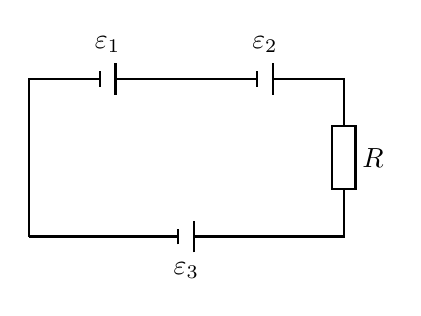
\begin{tikzpicture}[thick, scale=1]
    % Zanjir asosi (yopiq to'rtburchak kontur)
    \draw (0,0) -- (0,2) -- (4,2) -- (4,0) -- (0,0);

    % Yuqorigi tok manbalari (E1 va E2)
    % E1 manbasi (chapda): qutblari - | +
    \fill[white] (0.9,1.9) rectangle (1.1,2.1);
    \draw (0.9,1.9) -- (0.9,2.1); % Qisqa chiziq (-)
    \draw (1.1,1.8) -- (1.1,2.2); % Uzun chiziq (+)
    \node[above] at (1,2.2) {$\varepsilon_1$};

    % E2 manbasi (o'ngda): qutblari - | +
    \fill[white] (2.9,1.9) rectangle (3.1,2.1);
    \draw (2.9,1.9) -- (2.9,2.1); % Qisqa chiziq (-)
    \draw (3.1,1.8) -- (3.1,2.2); % Uzun chiziq (+)
    \node[above] at (3,2.2) {$\varepsilon_2$};

    % O'ng tomondagi vertikal simda joylashgan rezistor (R)
    \fill[white] (3.8,0.6) rectangle (4.2,1.4);
    \draw (3.85,0.6) rectangle (4.15,1.4) node[midway, right, xshift=3pt] {$R$};

    % Pastki gorizontal simda joylashgan tok manbasi (E3)
    % E3 manbasi: qutblari - | +
    \fill[white] (1.9,-0.1) rectangle (2.1,0.1);
    \draw (1.9,-0.1) -- (1.9,0.1); % Qisqa chiziq (-)
    \draw (2.1,-0.2) -- (2.1,0.2); % Uzun chiziq (+)
    \node[below] at (2,-0.2) {$\varepsilon_3$};

\end{tikzpicture}

\begin{enumerate}[label=\Alph*)]
\item 1,5.
\item 2.
\item 3.
\item 12.
\item 6.
\end{enumerate}

\item Uchta tok manbai va bitta qarshilikdan rasmda ko‘rsatilgan elektr zanjir tuzilgan. Agar $\varepsilon_1=3,5$ V, $\varepsilon_2=1,5$ V, $\varepsilon_3=2$ V, $r_1=r_2=r_3=0,2~\Omega$, $R=4,4~\Omega$ bo‘lsa, qarshilikdan o‘tayotgan tok kuchi necha Amper?

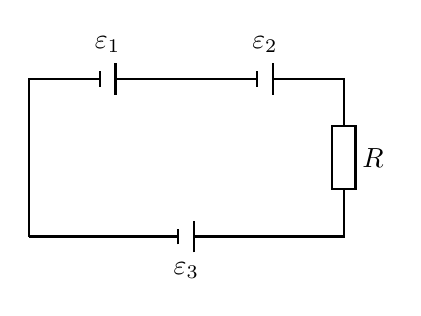
\begin{tikzpicture}[thick, scale=1]
    % Zanjir asosi (yopiq to'rtburchak kontur)
    \draw (0,0) -- (0,2) -- (4,2) -- (4,0) -- (0,0);

    % Yuqorigi tok manbalari (E1 va E2)
    % E1 manbasi (chapda): qutblari - | +
    \fill[white] (0.9,1.9) rectangle (1.1,2.1);
    \draw (0.9,1.9) -- (0.9,2.1); % Qisqa chiziq (-)
    \draw (1.1,1.8) -- (1.1,2.2); % Uzun chiziq (+)
    \node[above] at (1,2.2) {$\varepsilon_1$};

    % E2 manbasi (o'ngda): qutblari - | +
    \fill[white] (2.9,1.9) rectangle (3.1,2.1);
    \draw (2.9,1.9) -- (2.9,2.1); % Qisqa chiziq (-)
    \draw (3.1,1.8) -- (3.1,2.2); % Uzun chiziq (+)
    \node[above] at (3,2.2) {$\varepsilon_2$};

    % O'ng tomondagi vertikal simda joylashgan rezistor (R)
    \fill[white] (3.8,0.6) rectangle (4.2,1.4);
    \draw (3.85,0.6) rectangle (4.15,1.4) node[midway, right, xshift=3pt] {$R$};

    % Pastki gorizontal simda joylashgan tok manbasi (E3)
    % E3 manbasi: qutblari - | +
    \fill[white] (1.9,-0.1) rectangle (2.1,0.1);
    \draw (1.9,-0.1) -- (1.9,0.1); % Qisqa chiziq (-)
    \draw (2.1,-0.2) -- (2.1,0.2); % Uzun chiziq (+)
    \node[below] at (2,-0.2) {$\varepsilon_3$};

\end{tikzpicture}
\begin{enumerate}[label=\Alph*)]
\item 0,6.
\item 1,4.
\item 0,9.
\item 1,6.
\item 0,8.
\end{enumerate}

\item Sxemada $\varepsilon_1=2$ V, $\varepsilon_2=1$ V, $r_1=r_2=1~\Omega$, $R=2~\Omega$. Tashqi qarshilikdagi kuchlanish tushishini toping (V).

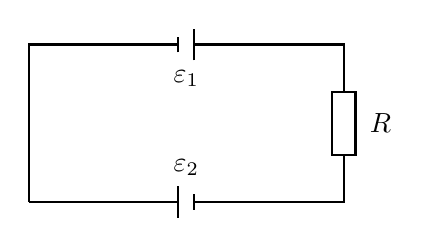
\begin{tikzpicture}[thick, scale=1]
    % Zanjir asosi (yopiq to'rtburchak kontur)
    \draw (0,0) -- (0,2) -- (4,2) -- (4,0) -- (0,0);

    % Yuqorigi tok manbai (E1) - Qutblari: - | + (chapdan o'ngga)
    \fill[white] (1.9,1.9) rectangle (2.1,2.1);
    \draw (1.9,1.9) -- (1.9,2.1); % Qisqa chiziq (-)
    \draw (2.1,1.8) -- (2.1,2.2); % Uzun chiziq (+)
    \node[below] at (2,1.8) {$\varepsilon_1$};

    % Pastki tok manbai (E2) - Qutblari: + | - (chapdan o'ngga)
    \fill[white] (1.9,-0.1) rectangle (2.1,0.1);
    \draw (1.9,-0.2) -- (1.9,0.2); % Uzun chiziq (+)
    \draw (2.1,-0.1) -- (2.1,0.1); % Qisqa chiziq (-)
    \node[above] at (2,0.2) {$\varepsilon_2$};

    

    % O'ng tomondagi rezistor (R2)
    \fill[white] (3.8,0.6) rectangle (4.2,1.4);
    \draw (3.85,0.6) rectangle (4.15,1.4);
    \node[right] at (4.2,1) {$R$};

\end{tikzpicture}
\begin{enumerate}[label=\Alph*)]
\item 0,5.
\item 1.
\item 1,5.
\item 2.
\item 3.
\end{enumerate}

\item Kondensatorlardagi kuchlanishlar qanday (V)? $\varepsilon_1=12$ V; $\varepsilon_2=13$ V; $C_1=3~\mu$F; $C_2=7~\mu$F.

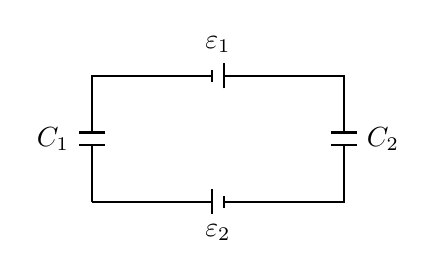
\begin{tikzpicture}[thick, scale=0.8]
    % Zanjir asosi (yopiq to'rtburchak kontur)
    \draw (0,0) -- (0,2) -- (4,2) -- (4,0) -- (0,0);

    % Yuqorigi tok manbai (E1) - Qutblari: - | +
    \fill[white] (1.9,1.9) rectangle (2.1,2.1);
    \draw (1.9,1.9) -- (1.9,2.1); % Qisqa chiziq (-)
    \draw (2.1,1.8) -- (2.1,2.2); % Uzun chiziq (+)
    \node[above] at (2,2.2) {$\varepsilon_1$};

    % Pastki tok manbai (E2) - Qutblari: + | -
    \fill[white] (1.9,-0.1) rectangle (2.1,0.1);
    \draw (1.9,-0.2) -- (1.9,0.2); % Uzun chiziq (+)
    \draw (2.1,-0.1) -- (2.1,0.1); % Qisqa chiziq (-)
    \node[below] at (2,-0.2) {$\varepsilon_2$};

    % Chap tomondagi kondensator (C1)
    \fill[white] (-0.1,0.9) rectangle (0.1,1.1);
    \draw (-0.2,0.9) -- (0.2,0.9); % Pastki plastinka
    \draw (-0.2,1.1) -- (0.2,1.1); % Yuqori plastinka
    \node[left] at (-0.2,1) {$C_1$};

    % O'ng tomondagi kondensator (C2)
    \fill[white] (3.9,0.9) rectangle (4.1,1.1);
    \draw (3.8,0.9) -- (4.2,0.9); % Pastki plastinka
    \draw (3.8,1.1) -- (4.2,1.1); % Yuqori plastinka
    \node[right] at (4.2,1) {$C_2$};

\end{tikzpicture}
\begin{enumerate}[label=\Alph*)]
\item 6,5; 18,5.
\item 7; 18.
\item 18; 7.
\item 17,5; 7,5.
\item 24; 1.
\end{enumerate}

\item Zanjirga ulangan $C_1$ va $C_2$ sig‘imli kondensatorlarning $q_1$ va $q_2$ zaryadlarini topilsin.

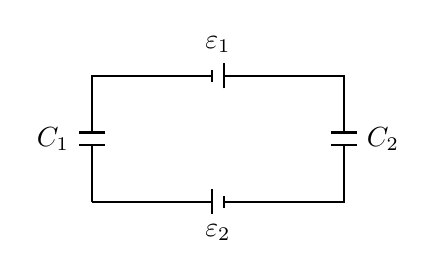
\begin{tikzpicture}[thick, scale=0.8]
    % Zanjir asosi (yopiq to'rtburchak kontur)
    \draw (0,0) -- (0,2) -- (4,2) -- (4,0) -- (0,0);

    % Yuqorigi tok manbai (E1) - Qutblari: - | +
    \fill[white] (1.9,1.9) rectangle (2.1,2.1);
    \draw (1.9,1.9) -- (1.9,2.1); % Qisqa chiziq (-)
    \draw (2.1,1.8) -- (2.1,2.2); % Uzun chiziq (+)
    \node[above] at (2,2.2) {$\varepsilon_1$};

    % Pastki tok manbai (E2) - Qutblari: + | -
    \fill[white] (1.9,-0.1) rectangle (2.1,0.1);
    \draw (1.9,-0.2) -- (1.9,0.2); % Uzun chiziq (+)
    \draw (2.1,-0.1) -- (2.1,0.1); % Qisqa chiziq (-)
    \node[below] at (2,-0.2) {$\varepsilon_2$};

    % Chap tomondagi kondensator (C1)
    \fill[white] (-0.1,0.9) rectangle (0.1,1.1);
    \draw (-0.2,0.9) -- (0.2,0.9); % Pastki plastinka
    \draw (-0.2,1.1) -- (0.2,1.1); % Yuqori plastinka
    \node[left] at (-0.2,1) {$C_1$};

    % O'ng tomondagi kondensator (C2)
    \fill[white] (3.9,0.9) rectangle (4.1,1.1);
    \draw (3.8,0.9) -- (4.2,0.9); % Pastki plastinka
    \draw (3.8,1.1) -- (4.2,1.1); % Yuqori plastinka
    \node[right] at (4.2,1) {$C_2$};

\end{tikzpicture}

\begin{enumerate}[label=\Alph*)]
\item $q_1=q_2=\dfrac{C_1C_2}{C_1+C_2}(\varepsilon_1+\varepsilon_2)$.
\item $q_1=q_2=\dfrac{C_1C_2}{C_1+C_2}(\varepsilon_1-\varepsilon_2)$.
\item $q_1=\dfrac{C_1}{C_1+C_2}(\varepsilon_1-\varepsilon_2),\quad
q_2=\dfrac{C_1}{C_1+C_2}(\varepsilon_2-\varepsilon_1)$.
\item $q_1=(C_1+C_2)(\varepsilon_1+\varepsilon_2),\quad
q_2=(C_1+C_2)(\varepsilon_1+\varepsilon_2)$.
\item $q_1=\dfrac{C_1}{C_1+C_2}(\varepsilon_1+\varepsilon_2),\quad
q_2=\dfrac{C_2}{C_1+C_2}(\varepsilon_1+\varepsilon_2)$.
\end{enumerate}


\item EYK’i $4,5$ V, ichki qarshiligi $1,5~\Omega$ bo‘lgan $5$ ta tok manbai parallel ulangan. Zanjirning to‘la EYK’i necha Volt?
\begin{enumerate}[label=\Alph*)]
\item 4,5.
\item 9.
\item 13,5.
\item 18.
\item 22,5.
\end{enumerate}

\item EYK’i $12$ V va ichki qarshiligi $3~\Omega$ dan bo‘lgan $6$ ta bir xil element parallel ulab, batareya hosil qilindi. Agar shu batareyaga $5,5~\Omega$ tashqi qarshilik ulansa, unda qanday tok kuchi hosil bo‘ladi (A)?
\begin{enumerate}[label=\Alph*)]
\item 0,5.
\item 1.
\item 1,5.
\item 2.
\item 3.
\end{enumerate}

\item EYK’i $12$ V, ichki qarshiligi $1~\Omega$ bo‘lgan $10$ ta tok manbai o‘zaro parallel ulab, batareya hosil qilindi. Shu batareyaga qarshiligi $5,9~\Omega$ bo‘lgan rezistor ulansa, undagi tok kuchi qanday bo‘ladi (A)?
\begin{enumerate}[label=\Alph*)]
\item 8.
\item 6.
\item 4.
\item 3.
\item 2.
\end{enumerate}

\item Uchta galvanik element va ikkita rezistordan rasmda ko‘rsatilgandek ulandi. Agar $R=12~\Omega$, $r=1,5~\Omega$ bo‘lsa, zanjirning umumiy qarshiligi necha $\Omega$?

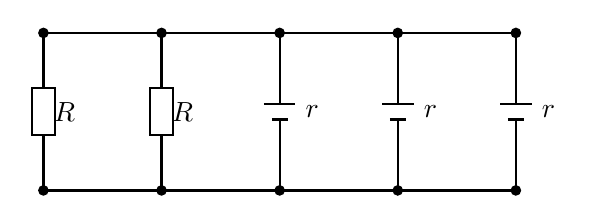
\begin{tikzpicture}[thick, scale=1]
    % Gorizontal magistral simlar (tugunlarni bog'laydi)
    \draw (0,2) -- (6,2);
    \draw (0,0) -- (6,0);

    % Ikkita parallel rezistor (R)
    \draw (0,2) -- (0,0);
    \fill[white] (-0.2,0.7) rectangle (0.2,1.3);
    \draw (-0.15,0.7) rectangle (0.15,1.3) node[midway, right] {$R$};

    \draw (1.5,2) -- (1.5,0);
    \fill[white] (1.3,0.7) rectangle (1.7,1.3);
    \draw (1.35,0.7) rectangle (1.65,1.3) node[midway, right] {$R$};

    % Uchta parallel tok manbai (har biri r ichki qarshilikka ega)
    % 1-manba
    \draw (3,2) -- (3,1.1);
    \draw (3,0.9) -- (3,0);
    \draw (2.8,1.1) -- (3.2,1.1); % Uzun chiziq (+)
    \draw (2.9,0.9) -- (3.1,0.9); % Qisqa chiziq (-)
    \node[right] at (3.2,1) {$r$};

    % 2-manba
    \draw (4.5,2) -- (4.5,1.1);
    \draw (4.5,0.9) -- (4.5,0);
    \draw (4.3,1.1) -- (4.7,1.1); % Uzun chiziq (+)
    \draw (4.4,0.9) -- (4.6,0.9); % Qisqa chiziq (-)
    \node[right] at (4.7,1) {$r$};

    % 3-manba
    \draw (6,2) -- (6,1.1);
    \draw (6,0.9) -- (6,0.9) -- (6,0);
    \draw (5.8,1.1) -- (6.2,1.1); % Uzun chiziq (+)
    \draw (5.9,0.9) -- (6.1,0.9); % Qisqa chiziq (-)
    \node[right] at (6.2,1) {$r$};

    % Tugun nuqtalari
    \foreach \x in {0,1.5,3,4.5,6} {
        \filldraw (\x,2) circle (1.5pt);
        \filldraw (\x,0) circle (1.5pt);
    }

\end{tikzpicture}

\begin{enumerate}[label=\Alph*)]
\item 2,3.
\item 6,5.
\item 1,2.
\item 7,5.
\item 13,5.
\end{enumerate}

\item EYK’lari $2,2$ V va ichki qarshiliklari $4~\Omega$ bo‘lgan ikki doimiy tok manbai bir xil qutblari bilan ulangan. Bu manbalar batareyasini qanday teng kuchli bir manba bilan almashtirish mumkin?
\begin{enumerate}[label=\Alph*)]
\item $\varepsilon=2,2$ V; $r=2,4~\Omega$.
\item $\varepsilon=4,4$ V; $r=2~\Omega$.
\item $\varepsilon=4,4$ V; $r=4~\Omega$.
\item $\varepsilon=2,2$ V; $r=2~\Omega$.
\item $\varepsilon=2,2$ V; $r=1~\Omega$.
\end{enumerate}

\item Qanday sharoitda $n$ element ketma-ket va parallel ulanganda, tok kuchi o‘zaro teng bo‘ladi?
\begin{enumerate}[label=\Alph*)]
\item $R=2r$.
\item $R=1,5r$.
\item $r=1,5R$.
\item $r=R$.
\item TJY.
\end{enumerate}

\item EYK’lari bir xil va ichki qarshiliklari $r$ bo‘lgan $n$ ta o‘zgarmas tok manbalari tashqi $R$ qarshilikka oldin parallel, keyin ketma-ket ulandi. Bu ikki hol uchun tashqi zanjirdagi tok kuchlarining nisbatini topilsin.
\begin{enumerate}[label=\Alph*)]
\item $n$.
\item $\dfrac{nR+r}{R+r}$.
\item $\dfrac{R+nr}{nR+r}$.
\item $\dfrac{nr}{R+r}$.
\item $\dfrac{R+nr}{nR-r}$.
\end{enumerate}

\item Aynan bir xil $n$ ta galvanik elementlarni ketma-ket va parallel ulangan hollarda bir xil o‘tkazgichdan o‘tayotgan tok kuchi bir xil bo‘lishi uchun quyidagi shartlardan qaysi biri bajarilishi lozim? $R$ -- tashqi zanjir qarshiligi, $r$ -- bir elementning ichki qarshiligi.
\begin{enumerate}[label=\Alph*)]
\item $R=r/2$.
\item $R=r/2$.
\item $R=r$.
\item $R=r/n$.
\item $R=nr$.
\end{enumerate}

\item Sxemada EYK’lar $\varepsilon_1=3$ V va $\varepsilon_2=2$ V, ichki qarshiliklar $r=0,5~\Omega$ bo‘lsa, voltmetr necha Voltni ko‘rsatadi? $R_v=\infty$.

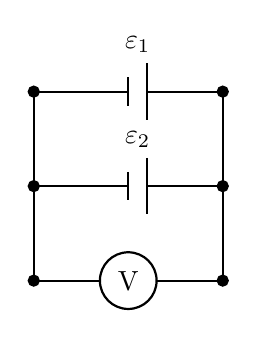
\begin{tikzpicture}[thick, scale=1.2]
    % Chap va o'ng vertikal magistral simlar
    \draw (0,0) -- (0,2);
    \draw (2,0) -- (2,2);

    % 1-tarmoq (yuqorida): epsilon1 va r
    \draw (0,2) -- (1,2);
    \draw (1,2.15) -- (1,1.85); % Qisqa chiziq (-)
    \draw (1.2,2.3) -- (1.2,1.7); % Uzun chiziq (+)
    \draw (1.2,2) -- (2,2);
    
    
    \node[above] at (1.1,2.3) {$\varepsilon_1$};

    % 2-tarmoq (o'rtada): epsilon2 va r
    \draw (0,1) -- (1,1);
    \draw (1,1.15) -- (1,0.85); % Qisqa chiziq (-)
    \draw (1.2,1.3) -- (1.2,0.7); % Uzun chiziq (+)
    \draw (1.2,1) -- (2,1);
    \node[above] at (1.1,1.3) {$\varepsilon_2$};

    % 3-tarmoq (pastda): Voltmetr
    \draw (0,0) -- (0.7,0);
    \draw (1.3,0) -- (2,0);
    \draw (1,0) circle (0.3) node {V};
   
    % Tugun nuqtalari
    \filldraw (0,1) circle (1.5pt);
    \filldraw (2,1) circle (1.5pt);
    \filldraw (0,2) circle (1.5pt);
    \filldraw (2,2) circle (1.5pt);
    \filldraw (0,0) circle (1.5pt);
    \filldraw (2,0) circle (1.5pt);

\end{tikzpicture}

\begin{enumerate}[label=\Alph*)]
\item 1.
\item 2,5.
\item 2.
\item 3.
\item 5.
\end{enumerate}

\item Sxemada EYK’lar $\varepsilon_1=3$ V va $\varepsilon_2=2$ V, ichki qarshiliklar $r=0,5~\Omega$ bo‘lsa, voltmetr necha Voltni ko‘rsatadi? $R_v=\infty$.

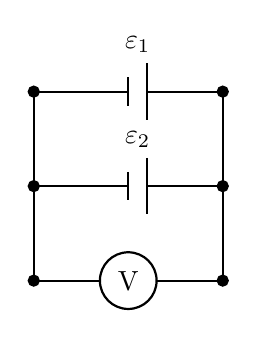
\begin{tikzpicture}[thick, scale=1.2]
    % Chap va o'ng vertikal magistral simlar
    \draw (0,0) -- (0,2);
    \draw (2,0) -- (2,2);

    % 1-tarmoq (yuqorida): epsilon1 va r
    \draw (0,2) -- (1,2);
    \draw (1,2.15) -- (1,1.85); % Qisqa chiziq (-)
    \draw (1.2,2.3) -- (1.2,1.7); % Uzun chiziq (+)
    \draw (1.2,2) -- (2,2);
    
    
    \node[above] at (1.1,2.3) {$\varepsilon_1$};

    % 2-tarmoq (o'rtada): epsilon2 va r
    \draw (0,1) -- (1,1);
    \draw (1,1.15) -- (1,0.85); % Qisqa chiziq (-)
    \draw (1.2,1.3) -- (1.2,0.7); % Uzun chiziq (+)
    \draw (1.2,1) -- (2,1);
    \node[above] at (1.1,1.3) {$\varepsilon_2$};

    % 3-tarmoq (pastda): Voltmetr
    \draw (0,0) -- (0.7,0);
    \draw (1.3,0) -- (2,0);
    \draw (1,0) circle (0.3) node {V};
   
    % Tugun nuqtalari
    \filldraw (0,1) circle (1.5pt);
    \filldraw (2,1) circle (1.5pt);
    \filldraw (0,2) circle (1.5pt);
    \filldraw (2,2) circle (1.5pt);
    \filldraw (0,0) circle (1.5pt);
    \filldraw (2,0) circle (1.5pt);

\end{tikzpicture}

\begin{enumerate}[label=\Alph*)]
\item 0,5.
\item 1.
\item 2.
\item 3.
\item 5.
\end{enumerate}

\item Elektr yurituvchi kuchlari teng, ichki qarshiliklari $2$ marta farq qiladigan tok manbalari rasmdagidek ulangan. Voltmetrning ko‘rsatishini toping. $R_v=\infty$.

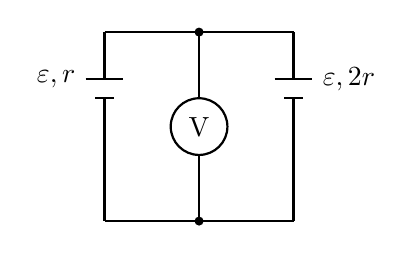
\begin{tikzpicture}[thick, scale=1.2]
    % Gorizontal magistral simlar
    \draw (0,2) -- (2,2);
    \draw (0,0) -- (2,0);

    % Chap tarmoq: epsilon va r
    \draw (0,2) -- (0,1.5);
    \draw (-0.2,1.5) -- (0.2,1.5); % Uzun chiziq (+)
    \draw (-0.1,1.3) -- (0.1,1.3); % Qisqa chiziq (-)
    \draw (0,1.3) -- (0,0);
    \node[left] at (-0.2,1.5) {$\varepsilon,r$};

    % Markaziy tarmoq: Voltmetr
    \draw (1,2) -- (1,1.3);
    \draw (1,1) circle (0.3) node {V};
    \draw (1,0.7) -- (1,0);

    % O'ng tarmoq: epsilon va 2r
    \draw (2,2) -- (2,1.5);
    \draw (1.8,1.5) -- (2.2,1.5); % Uzun chiziq (+)
    \draw (1.9,1.3) -- (2.1,1.3); % Qisqa chiziq (-)
    \draw (2,1.3) -- (2,0);
    \node[right] at (2.2,1.5) {$\varepsilon, 2r$};

    % Tugun nuqtalari
    \filldraw (1,2) circle (1pt);
    \filldraw (1,0) circle (1pt);

\end{tikzpicture}

\begin{enumerate}[label=\Alph*)]
\item 0.
\item $\varepsilon/2$.
\item $\varepsilon$.
\item $2\varepsilon/3$.
\item $\varepsilon/3$.
\end{enumerate}

\item EYuK’i $1,5$ V va $2$ V bo‘lgan elementlar bir xil ishorali qutblari bilan ulangan. Batareya klemmalariga ulangan voltmetr $1,7$ V kuchlanishni ko‘rsatdi. Elementlar ichki qarshiliklarining nisbatini toping.
\begin{enumerate}[label=\Alph*)]
\item 1.
\item $2/3$.
\item 2.
\item $1/3$.
\item 3.
\end{enumerate}

\item EYK’lari $\varepsilon_1$ va $\varepsilon_2$ bo‘lgan manbalar bir xil qutblari bilan o‘zaro parallel ulangan. Agar manbalarning ichki qarshiliklari teng bo‘lsa, manba qutblaridagi potensiallar farqi qanday?
\begin{enumerate}[label=\Alph*)]
\item $\varepsilon_1+\varepsilon_2$.
\item $(\varepsilon_1-\varepsilon_2)/2$.
\item 0.
\item $\varepsilon_1-\varepsilon_2$.
\item $(\varepsilon_1+\varepsilon_2)/2$.
\end{enumerate}

\end{enumerate}

\begin{table}[h!]
\centering
\begin{tabular}{|c|c|c|c|c|c|c|c|c|c|}
\hline
1e & 2e & 3d & 4b & 5c & 6e & 7c & 8b & 9c & 10a \\ \hline
11b & 12e & 13c & 14d & 15a & 16a & 17d & 18e & 19b & 20d \\ \hline
21d & 22c & 23c & 24b & 25a & 26c & 27b & 28e &  &  \\ \hline
\end{tabular}
\end{table}



